
% controlled-assessments.tex - Our first LaTeX example!

%%%%%%%%%%%%%%%%%%%%%%%%%%%%%%%%%%%%%%%%%
% Beamer Presentation
% LaTeX Template
% Version 1.0 (10/11/12)
%
% This template has been downloaded from:
% http://www.LaTeXTemplates.com
%
% License:
% CC BY-NC-SA 3.0 (http://creativecommons.org/licenses/by-nc-sa/3.0/)
%
%%%%%%%%%%%%%%%%%%%%%%%%%%%%%%%%%%%%%%%%%

%----------------------------------------------------------------------------------------
%	PACKAGES AND THEMES
%----------------------------------------------------------------------------------------

\documentclass{beamer}
\mode<presentation> {

% The Beamer class comes with a number of default slide themes
% which change the colors and layouts of slides. Below this is a list
% of all the themes, uncomment each in turn to see what they look like.

%\usetheme{default}
%\usetheme{AnnArbor}
%\usetheme{Antibes}
%\usetheme{Bergen}
%\usetheme{Berkeley}
%\usetheme{Berlin}
%\usetheme{Boadilla}
%\usetheme{CambridgeUS}
%\usetheme{Copenhagen}
%\usetheme{Darmstadt}
%\usetheme{Dresden}
%\usetheme{Frankfurt}
%\usetheme{Goettingen}
%\usetheme{Hannover}
%\usetheme{Ilmenau}
%\usetheme{JuanLesPins}
%\usetheme{Luebeck}
\usetheme{Madrid}
%\usetheme{Malmoe}
%\usetheme{Marburg}
%\usetheme{Montpellier}
%\usetheme{PaloAlto}
%\usetheme{Pittsburgh}
%\usetheme{Rochester}
%\usetheme{Singapore}
%\usetheme{Szeged}
%\usetheme{Warsaw}

% As well as themes, the Beamer class has a number of color themes
% for any slide theme. Uncomment each of these in turn to see how it
% changes the colors of your current slide theme.
\definecolor{mypurplish}{rgb}{0.3, 0.12, 0.4}
%\usecolortheme{albatross}
%\usecolortheme{beaver}
%\usecolortheme{beetle}
%\usecolortheme{crane}
%\usecolortheme{dolphin}
%\usecolortheme{dove}
%\usecolortheme{fly}
%\usecolortheme{lily}
%\usecolortheme{orchid}
%\usecolortheme{rose}
%\usecolortheme{seagull}
%\usecolortheme{seahorse}
%\usecolortheme{spruce}
%\usecolortheme{whale}
%\usecolortheme{wolverine}
\usecolortheme[named=mypurplish]{structure}
%\setbeamertemplate{footline} % To remove the footer line in all slides uncomment this line
%\setbeamertemplate{footline}[page number] % To replace the footer line in all slides with a simple slide count uncomment this line

%\setbeamertemplate{navigation symbols}{} % To remove the navigation symbols from the bottom of all slides uncomment this line
}
\usepackage{graphicx} % Allows including images
\usepackage{booktabs} % Allows the use of \toprule, \midrule and \bottomrule in tables
\usepackage{tikz}



\newcommand\RBox[1]{%
  \tikz\node[draw,rounded corners,align=center,] {#1};%
}  
\usepackage{color}
\usepackage{listings}
\usepackage{setspace}

\usepackage[framemethod=tikz]{mdframed}



\definecolor{Code}{rgb}{0,0,0}
\definecolor{Decorators}{rgb}{0.2,0.2,0.2}
\definecolor{Numbers}{rgb}{0.5,0,0}
\definecolor{MatchingBrackets}{rgb}{0.25,0.5,0.5}
\definecolor{Keywords}{rgb}{0,0,1}
\definecolor{self}{rgb}{1,0,0}
\definecolor{Strings}{rgb}{0,0.63,0}
\definecolor{Comments}{rgb}{0,0.63,1}
\definecolor{Backquotes}{rgb}{0,0.2,0}
\definecolor{Classname}{rgb}{0,0,1}
\definecolor{FunctionName}{rgb}{1,0,1}
\definecolor{Operators}{rgb}{0,0,0}
\definecolor{Background}{rgb}{0.95,0.95,0.95}


            
\lstset{
numbers=left,
numberstyle=\footnotesize,
numbersep=1em,
xleftmargin=1em,
framextopmargin=2em,
framexbottommargin=2em,
showspaces=false,
showtabs=false,
showstringspaces=false,
frame=l,
tabsize=4,
breaklines=true,
postbreak=\raisebox{0ex}[0ex][0ex]{\ensuremath{\color{red}\hookrightarrow\space}},
% Basic
basicstyle=\ttfamily\small\setstretch{1},
backgroundcolor=\color{Background},
language=Python,
% Comments
commentstyle=\color{Comments},
% Strings
stringstyle=\color{Strings},
morecomment=[s][\color{Strings}]{"""}{"""},
morecomment=[s][\color{Strings}]{'''}{'''},
% keywords
morekeywords={import,from,class,def,for,while,if,is,in,elif,else,not,and,or,print,break,continue,return,True,False,None,access,as,,del,except,exec,finally,global,import,lambda,pass,print,raise,try,assert},
keywordstyle={\color{Keywords}\bfseries},
% additional keywords
morekeywords={[2]@invariant},
keywordstyle={[2]\color{Decorators}\slshape},
emph={self},
emphstyle={\color{self}\slshape},
%
}{}

\title[GUIs]{Python in Education      }
\author[Dave Ames]{Dave Ames}
\institute[CAS]{Computing At School}


\begin{document}

{
  \usebackgroundtemplate{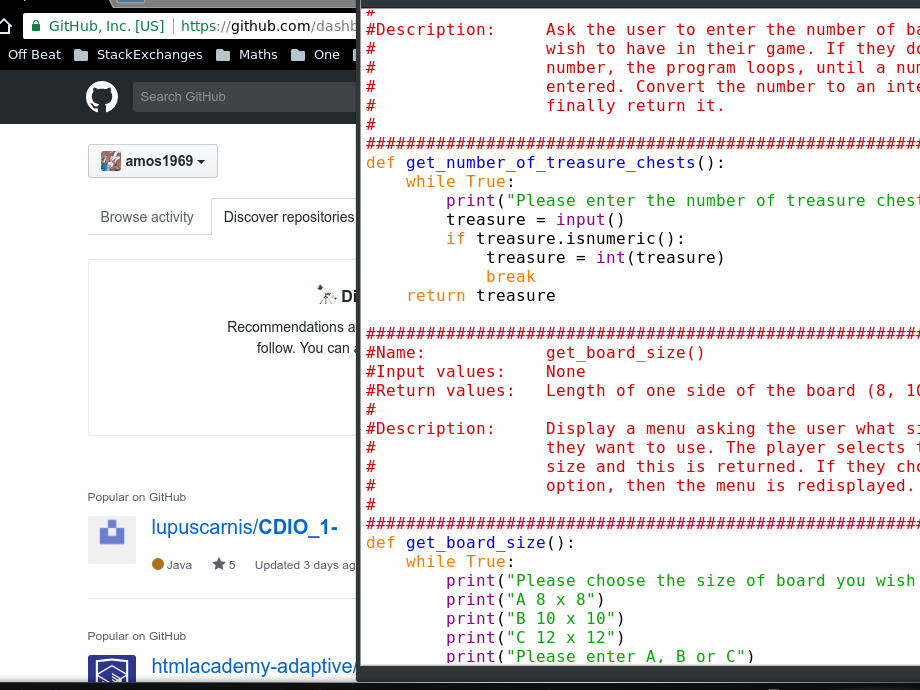
\includegraphics[width=1.0\paperwidth]{front_slide.png}}
  \begin{frame}[plain]
    \vspace{2cm}
    \centering
\begin{mdframed}[tikzsetting={draw=mypurplish,fill=white,fill opacity=0.8,
               line width=3pt},backgroundcolor=none,leftmargin=20,
               rightmargin=20,innertopmargin=8pt,roundcorner=15pt]
               {\huge \inserttitle} \\
               \insertauthor  \hspace{0.4cm}  (\insertinstitute) \hspace{0.3cm}  \insertdate \\
               \href{mailto:dave.ames@computingatschool.org.uk}{E: dave.ames@computingatschool.org.uk} \hspace{0.2cm}
               \href{http://twitter.com/davidames}{T: @DavidAmes}
               
             \end{mdframed}
\end{frame}
}




\section{Main part}



\begin{frame}
\frametitle{My background}
\subsection{My background}

\begin{itemize}
  \pause
\item I learnt to program in Sinclair BASIC on a 48k ZX Spectrum around 1982/3
  \pause
\item I did a Mode 3 CSE in Computer Science in the Lower Sixth (1986)
  \pause
\item Which was done in Basic on the TRS80
  \pause
\item Did a Maths Degree (some programming but I skipped that module)
\pause
\item Did my teacher training 1991/92 (elements of programming in LOGO)
\pause
\item Started working as a Maths Teacher in January 1993
  \pause
\item Bought an Amiga 1200 soon after (played with a programming language called AMOS which was a variant of Basic) 
  \pause
\item I used that until about 1997 but didn't move on to a PC initially (PCs were about \pounds1000+)
\pause
\item Got a PC around 2000/2001 in the second wave of the \textbf{Computers for Teacher} Scheme
\pause
\item Started playing with programming languages and Linux within about 6 months of getting it
\end{itemize}

\end{frame}

\begin{frame}
\frametitle{Background Pt2}
\subsection{Background Pt2}

\begin{itemize}
\pause
\item Settled on C++ as lots of Applications and Games seemed to be using it
\pause
\item Taught myself on and off for the next few years, but got bogged down and decided I needed external help (2004)
\pause
\item Discovered that Bolton Uni (still Bolton Institute of Higher Ed) did a Part Time Degree and guaranteed that every
  module would be accessible in the evenings over the duration of the course.
\pause
\item At some point in the previous 3-4 years I'd printed off a load of chapters from the Python documentation and
  worked through some
\pause
\item Spent the next 4 1/2 years learning C++, SQL stuff, various theory modules and a bit of VB6.
\pause
\item At this point I was still doing very little with regards to Python.
\end{itemize}
\end{frame}

\begin{frame}
  \frametitle{Background Pt3}
  \subsection{Background Pt3}

  \begin{itemize}
    \pause
  \item During the final six months of my degree I became responsible for my school's VLE and Website
    \pause
  \item We chose Moodle for the VLE and I chose to create a Django based website for some reason
    \pause
  \item Basically I'd played with Python (PyQt and Pygame I think) and wanted an excuse to use it for a project
    \pause
  \item The site used Django 0.8 I think and content was updated weekly until 2013, when they replaced it with
    something related to the new VLE they bought in.
    \pause
  \item By this point though the curriculum had changed and my school asked me to change from teaching Maths to
    Computing 
  \end{itemize}
\end{frame}

\begin{frame}
  \frametitle{The Change to Computing}
  \subsection{The Change to Computing}

  \begin{itemize}
    \pause
  \item From the early 90s onwards IT and ICT as a subject began to develop, initially as part of Design Technology then
    as a discrete subject
    \pause
  \item By 2010 or so it had sort of crystallised into using Microsoft products to solve a project focused problem (Plan
    a School Prom etc)
    \pause
  \item As an outsider looking in, it was very, very... \pause \textbf{dull!}
    \pause
  \item Late 2011 Ian Livingstone published the `\textbf{Next: Gen} report.
    \pause
  \item In early 2012 the Royal Society published the \textbf{Shutdown, Restart?} report.
    \pause
  \item Around the same time a senior executive at Google made a very public speech criticising ICT in this country as
    not fit for purpose
    \pause
  \item Michael Gove announced the dis-application of the National Curriculum for ICT from September 2012, with a new
    Computer Science focused curriculum to replace it from 2014.
    \pause
  \item Which meant in theory we could teach whatever we liked!
  \end{itemize}
\end{frame}

\begin{frame}
  \frametitle{A New Era of Computing in Schools?}
  \subsection{A New Era of Computing in Schools?}
  \begin{itemize}
    \pause
  \item Over the next few years many schools began to teach what they thought a new Computing curriculum would look
    like
    \pause
  \item Some continued with their existing ICT curricula
    \pause
  \item Some decided they no longer needed to teach anything ICT related and killed all of their courses
    \pause
  \item Most schools that took to Computing/Computer Science went down one of two routes:
    \pause
    \begin{itemize}
      \pause
    \item They already did A Level, took whatever their language of choice was there and worked backwards
      \pause
    \item They didn't do any programming already and chose to do something which appeared to have lots of support
    \end{itemize}
    \pause
  \item The latter ones often found their way to Python, the earlier ones mostly focused on the .net languages with
    Small Basic leading them into it.
  \end{itemize}
 
\end{frame}

  

\end{document}

%%% Local Variables:
%%% mode: latex
%%% TeX-master: t
%%% End:
